\documentclass[../Main.tex]{subfiles}
\begin{document}

Today we have a great variety of free open-source tools for NN purposes and its number is increasing with the growth of AI and ML. Development of neural networks, mobile application or server is full of nuances, unexperienced programmer may encounter many troubles since not everything can be easily tracked. However most problems can be solved by good Internet research. Therefore, it is highly significant to choose the up-to-date tools with well-prepared documentation and active communities. Technologies we have chosen allowed us to focus on core concepts instead of struggling with implementation or configuration.

\subsection{Neural Network}

    \subsubsection{PyTorch}
        PyTorch is an open-source machine learning library created by Facebook and broadly used in the field of computer vision. Released in 2016 rapidly gained popularity among researchers and developers. PyTorch is not an another Python binding into a C++ framework. It uses core Python concepts like structures, classes or conditions, so integrates easily with the rest of Python ecosystem. Library provides all necessary tools for developing and training neural network based on deep learning models.
        
        Two main features of this package are:
        \begin{itemize}
            \item Strong GPU acceleration during computation of tensors
            \item Neural networks built on a tape-based autograd system
        \end{itemize}
        
        We decided to pick out PyTorch instead of TensorFlow (the main and actually the only alternative) due to several reasons. Firstly, TensorFlow was becoming more and more complex for machine learning beginners, where the PyTorch is based on basic and familiar programming paradigms. New version of TF (2.0) solves this problem, but was released after we had started working on the project. Moreover, the documentation is also pretty straightforward and helpful for newcomers. And finally, plenty of style transfer approaches are built on PyTorch. Including the network we adopt. 
        \bartek{add biblio: https://pytorch.org/docs/stable/index.html}
        
    \subsubsection{TensorRT}
    TensorRT is a SDK for deep learing interface created by NVIDIA and design for graphic cards from this company. It allowed optimalize neutral network 
    
    \subsubsection{OpenCV}
    Open Source Computer Vision Library is an open-source library for the machine learning, image processing and so on. It includes dozens of computer vision algorithms adjusted for easy use. Althought written in C++, OpenCV has Python bindings and provides support for Machine Learning libraries like PyTorch.  By using it, one can process images and videos to detect objects, apply filters, analyze structure or perform reconstruction. OpenCV is designed to handle real-time vision applications and is curently developing full-featured CUDA interfaces.
    \bartek{describe what do we use it for}
    \bartek{add: https://docs.opencv.org/master/}
        
    \subsubsection{CUDA}
    todo
    
\newpage
\subsection{Server}
    Client-server communication is divided into two parts: video streaming and transferring filter specification data. The first part is maintained by server in WebRTC standard, whereas the second one is micro-server based on Flask. Both segments are written in Python and developed by open-source communities.

    \subsubsection{WebRTC}
    WebRTC is an open framework that enables Real Time Communication (RTC) in web browsesr and mobile apps via simple API. It provides tools to create peer-to-peer communication without any external plugins or programs. Standarized on API level by W3C \bartek{add hyperlink} and protocol level by IETF \bartek{add hyperlink} is widely used and supported by Google, Apple, Microsoft and main browser vendors. Given that our project and mobile application is cross-platfrom, we consider it as a key factor when chosing server technology.
    
    WebRTC architecture presented on Figure Figure \ref{fig:webrtc-public-diagram-for-website} contains two main layers: 
    \begin{itemize}
    \item C++ API - for browser makesrs implementing the Web API proposal
    \item Javascript Web API - for web developers building audio-video applications \\
    \end{itemize}
    
    \begin{figure}[h]
    \centering
    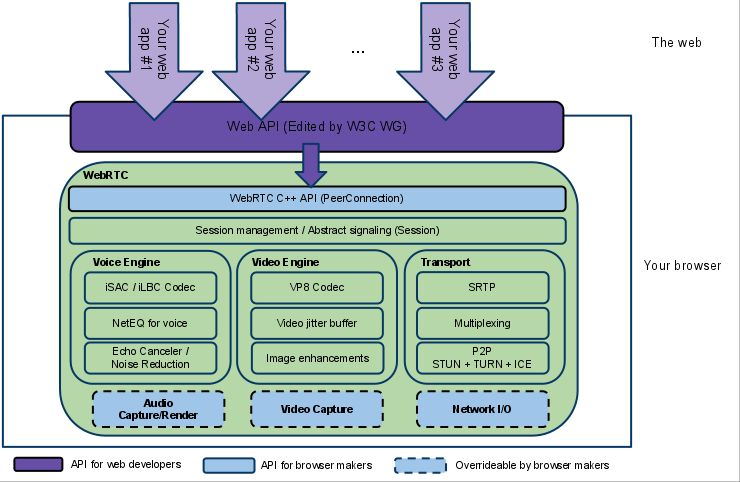
\includegraphics[width=0.7\textwidth]{webrtc-public-diagram-for-website}
    \caption{Overview of WebRTC architecture}
    \label{fig:webrtc-public-diagram-for-website}
    \end{figure}

    Comprehensive documentation and community creating many additional libraries make using this framework rather convenient. One of the most popular open-source libraries is \textbf{aiortc}.
    \bartek{
    photo: https://webrtc.org/architecture/
    biblio: https://webrtc.org
    }
    
    \subsubsection{Aiortc}
    \textit{aiortc} was developed as a 'WebRTC for Python'. Complexity (especially for beginners) and lack of Python bindings motivated authors of aiortc to design library and API which follow its Javascript counterpart. They pointed out that \bartek{add cite} 'WebRTC (...) is tightly coupled to a media stack, making it hard to plug in audio or video processing algorithms'. Our goal is to literally use the video processing algorithm, so we found this library and its examples extremely useful.
    We based our server on the aiortc example which performs video, audio and data channel establishing with a browser. It also allows to process streaming frames using OpenCV. 
        \bartek{biblio: https://aiortc.readthedocs.io/en/stable/}
    
    \subsubsection{Flask}
    Flask is so-called micro-framework with little dependencies to external libraries, which provides tools and technologies useful with building a small web application. It could be helpful for ones who want to create web pages, blogs or simple REST server. 
    Technically, Flask is based on:
    \begin{itemize}
    \item Werkzeug WSGI (Web Server Gateway Interface is a popular specification for a universal interface between the  server and the web app) - toolkit which implements requests-response objects, and some service functions
    \item Jinja2 template engine - template system helpful with rendering dynamic web pages
    \end{itemize}
    Flask itself does not support database handling, validation or extensive visual templates. Being lightweight is the factor we found crucial, since our server does not perform any complicated tasks. Running constantly in the background, it only has to:
    \begin{itemize}
    \item Receive POST request from mobile application containing filter specification 
    \item Encode filter image and parameters
    \item Assign it to the IP of sender and store in particular folder
    \item Send confirmation response to the mobile app
    \end{itemize}
    We also decided to write simple Flask client in order to test connection to the server.
    \bartek{biblio to add: http://flask.palletsprojects.com/en/1.1.x/}
    
    \subsubsection{Server flow}
    Aforementioned servers work separately and do not directly interfere with each other and could perform tasks asynchronously. In that way, many clients can upload filter image and parameters as well as stream video without delays. Every client is able to change filter params and start new stream in various order, but usual client-server flow is depicted on Figure \ref{fig:server-flow} \\
    \begin{figure}[h]
    \centering
    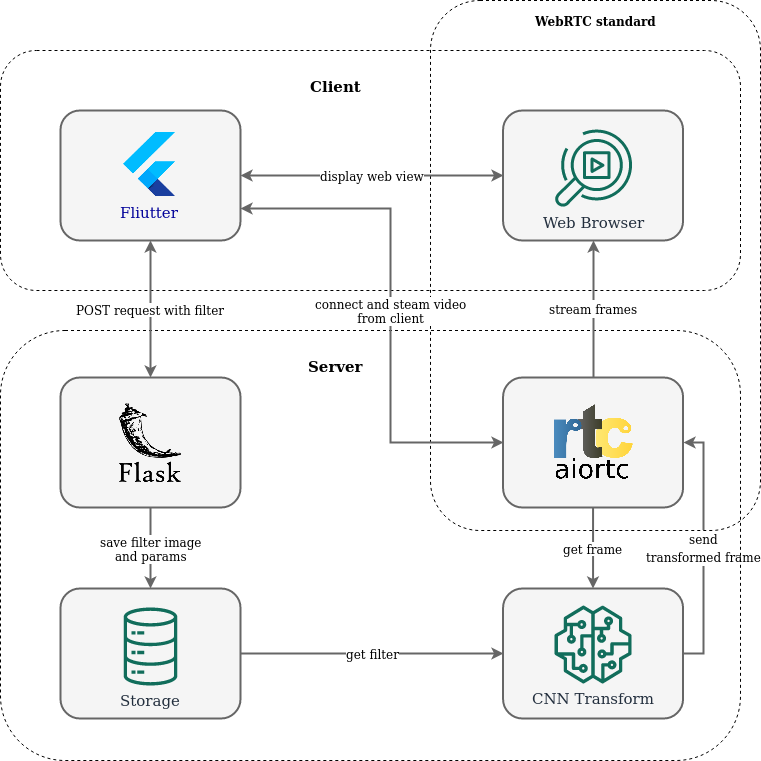
\includegraphics[width=0.7\textwidth]{server-flow}
    \caption{Client-server flow}
        \label{fig:server-flow}
    \end{figure}
    
    In a nutshell, when user selects filter style the following actions happen:
    \begin{enumerate}
    \item Mobile app send POST request to the Flask server running on port 5000 including JSON with three fields: filter image encoded in base64 format, filter benchmark value in float, boolean information about color preservation during process 
    \item Flask server performs tasks described in the section 5.2.3
    \item Mobile app ping server running on port 8080
    \item Server establishes RTC-peer connection with browser running inside app
    \item The stream is started - aiortc-based server catch frame and transform it using filter style image uploaded in advance from storage
    \item Transformed frame is added to RTC Media Stream Track and streamed back to the mobile browser
    \item Browser displays video using WebView component 
    \end{enumerate}
    
    When stream finishes or breaks (due to network error, application shutdown or any other error), server close connection gracefully but still stores last filter style parameters. If they are not specified during next stream or the POST request to the Flask server failes, the server uses saved ones. 
    
    \subsubsection{Alternative technologies}
    We had been trying several options before we chose to use aiortc. Our prime attempt was to adopt \textit{WebRTC Plugin for Flutter}. It is small project developed by Flutter community containing Javascript server and Flutter client. That seemed to be a perfect solution which could accelerate our work.
    However we encounter some obstacles in this undertaking. First of all, mentioned plugin is poorly documented and error-prone what is rather annoying combination. Secondly it works efficiently only over LAN network when we wish to connect to the server from any place. And the third thing is the communication crashes if the video is not streaming to/from Chrome browser. Nevertheless, the project is gathering greater community what makes it promising in the time of growing popularity of Flutter.
    \bartek{biblio to add:  https://github.com/cloudwebrtc/flutter-webrtc}
   
\newpage
\subsection{Mobile Application}
    This part describes the style tranfer clinet, which is mobile application 
    for Android systems. We will go through all features of the application and
    explain why we've choosen Flutter framework. 
    \subsubsection{Flutter}
        Today there are several frameworks which allow us to create mobile 
        applications for both Android and iOS simultaneously, 
        eg. React Native, Ionic, Xamarin.
        In 2015 Flutter joined this family and changed drasticly situation
        on mobile application scene. At the moment when we write this article,
        Flutter is the most popular multiplatform framework, which allow us to 
        create not only mobile applications but also web from single codebase.
    
    \subsubsection{Description}
        Flutter is framework created by Google but it's also an open source project 
        so everone can propose new fetures and improvments. 
        When we write Flutter application we use Dart language.
        Dart is also developed by Google and has C-style syntax.
        It runs's on Dart VM included in the SDK. 
        Very interesting feautre of Dart is that it can transcompile to JavaScript.
        This feature is 
    
    There are Material Design 
        icons, colors, typical UI interface elements like top and bottom bars,
        buttons, list, animations and much more. 
        It all makes creating app with "professional" look very easy.
        
        
    \subsubsection{Motivation}
        From the begining of our project we wanted to be able to develop new ideas
        very quickly.
        Python and PyTorch are technologies which definitely helped us keep high
        productivity during this time. First choise was Kotlin - new mordern programing 
        language for Android apps. Main advantages of Kotlin are:
            \begin{itemize}
                \item officialy supported by Google
                \item high performance - native application
                \item some great language features like null safety, readabilty or async functions
                \item we had some experience with this langauge
            \end{itemize}
            
        The main drawback of creating mobile apps with Kotlin is that creating 
        some simple things can often take much time and effort. 
        This was a main cause of rejecting this approach.
        We've looked for some other tools to create our clinet application and 
        we've found Flutter - relatively new tool framework from Google which 
        is still developing very quickly.
        The main advantage of Flutter is that you can develop your apps very 
        quckly beceause there are tons of ready, efficient and highly costumizable 
        widgets. There is also large community which creates new great widgets 
        add publishes them on official website so everyone can dowload them and use in project.
        You can also modify or build new widgets on top of it and then publish.
        If some widget would become very popular and usefull it will may be 
        include to official Flutter SDK. 
        Flutter also makes easy to create apps in beatiful Mateterial Design 
        style or it's iOS equivalent - Cupertino. 
        The main feature of Flutter, and always mentioned by Google is of course 
        creating apss for Android and iOS at the same time. 
        Our main goal was to create app for Android so we treated this feature like 
        an opened door. 
        Flutter is also declarative, react style framework which we prefere while
        creating user interface's. We've had previous experience with React on web
        so Flutter seemed easy to learn.  
        
    \subsubsection{Difficulties}



\biblio % Needed for referencing to working when compiling individual subfiles - Do not remove
\end{document}

